\setcounter{page}{1}
\section*{Zielsetzung}
In dem Versuch V27 soll der \emph{Zeeman-Effekt} experiementell beobachtet werden.
Hierzu wird die Aufspaltung der Energieniveaus einer Kadmium Spektrallampe
unter Einwirkung eines äußeren Magnetfeldes untersucht.

\section{Theorie}

\subsection{Magnetisches Moment und Energieaufspaltung}
\subsubsection{Magnetische Momente}
Aus der Quantenmechanik geht hervor, dass Elektronen neben ihrem Drehimpuls $\vec{l}$ auch einen
Eigendrehimpuls oder auch Spin genannt $\vec{s}$ besitzen. Charakterisiert werden die beiden Größen durch die
Quantenzahlen $l$ und $s$. Aus der Eigenwertgleichung resultiert:
\begin{align*}
\be{\vec{l}}&=\sqrt{l(l+1)}\hbar & l&=0,1,2,\dots,n-1\\
\be{\vec{s}}&=\sqrt{s(s+1)}\hbar & s&=\frac{1}{2}.
\end{align*}
Auf Grund der Ladung des Elektrons $\map{e}_0$ entstehen magnetische Momente, die
proportional zum Bohrschen Magneton $\map{\mu}_B$ sind und durch
\begin{equation}
  \label{eq:bohrsche_magneton}
  \map{\mu_B}:=-\frac{1}{2}\map{e}\ua{0} \frac{\hbar}{\map{m}\ua{0}}
\end{equation}
definiert werden. Die in Gleichung \eqref{eq:bohrsche_magneton} auftretende Größe $\map{m}_0$ ist die Elektronenmasse.
Für die magnetischen Momente ergeben sich die folgenden Definitionen:
\begin{align*}
  \vec{\mu}\ua{l}&=-\map{\mu_B}\frac{\vec{l}}{\hbar}=-\map{\mu_B}\sqrt{l(l+1)}\vec{e}\ua{\vec{l}} \\
  \vec{\mu}\ua{s}&=-\map{g_S}\map{\mu_B}\frac{\vec{s}}{\hbar}=-\map{g_S}\map{\mu_B}\sqrt{s(s+1)}\vec{e}\ua{\vec{s}}.
\end{align*}
Mit $\map{g_S}$ wird der Lande-Faktor des Elektrons bezeichnet und trägt den Wert $\map{g_S}\approx 2$.
Auf fallend ist, dass das magnetische Spinmoment $\vec{\mu}\ua{s}$ des Elektrons in etwa doppelt
so groß ist wie das magentische Bahnmoment $\vec{\mu}\ua{l}$.

\subsubsection{Wechselwirkung der Magnetischen Momente}

Bei dem Übergang zu Mehrelektronatomen müssen die Wechselwirkungen der Momente und Drehimpulse untereinander und
deren der einzelnen Elektronen untereinander unterschieden werden. Die Wechselwirkungen hängen im Wesentlichen
von der Kernladungszahl $Z$ ab.
Bei Atomen mit einer niedrigen Kernladungszahl ist die Wechselwirkung der Bahndrehimpulse $\vec{l}_i$ so groß, dass diese zu einem
Geasamtbahndrehimpuls $\vec{L}$ zusammengefasst werden können. Dieser wird definiert durch
\begin{equation*}
  \vec{L}=\sum_{i=1}^{Z} \vec{l}_i, \qquad \be{\vec{L}}=\sqrt{L(L+1)}\hbar.
\end{equation*}
Genauso gilt für den Gesamtspin
\begin{equation*}
  \vec{S}=\sum_{i=1}^{Z} \vec{s}_i, \qquad \be{\vec{S}}=\sqrt{S(S+1)}\hbar.
\end{equation*}
Auf Grund der Halbzahligkeit eines einzelnen Spins $\vec{s}_i$, kann auch $\vec{S}$ halbzahlige Werte annehmen.

Die jeweiligen Impulse besitzen auch zugehörige magnetische Momente:
\begin{align*}
  \be{\vec{\mu}}\ua{L}&=\map{\mu_B}\sqrt{L(L+1)}\\
  \be{\vec{\mu}}\ua{S}&=\map{g_S}\map{\mu_B}\sqrt{S(S+1)}.
\end{align*}

Unter der Prämisse, dass sich die Atome in keinem großen Magnetfeld befinden, ist es möglich einen Gesamtdrehimpuls $\vec{J}$ zu
definieren
\begin{align*}
  \vec{J}&=\vec{L}+\vec{S}\\
\shortintertext{mit}
\be{\vec{J}}&=\sqrt{J(J+1)}\hbar.
\end{align*}
Dieser Fall wird als \emph{LS-Kopplung} bezeichnet.
Neben der LS-Kopplung gibt es die \emph{jj-Kopplung}, die bei Atomen mit hoher Kernladungszahl auftritt.
Bei der jj-Kopplung ist die Wechselwirkung zwischen Spin und Bahndrehimpuls des Elektrons groß gegenüber der Wechselwirkung der $\vec{l}_i$ und
$\vec{s}_i$. Auf Grund dessen wird die Größe
\begin{equation*}
  \vec{j}_i=  \vec{l}_i+  \vec{s}_i
\end{equation*}
eingeführt. Das verwenden von $\vec{L}$ und $\vec{S}$ ist nicht mehr möglich.
Stattdessen existiert
\begin{equation*}
  \vec{J}=\sum_{i=1}^{Z} \vec{j}_i
\end{equation*}
der Gesamtdrehimpuls der Hülle.
Zwischen der LS-Kopplung und der jj-Kopplung gibt es einen kontinuierlichen Übergang.

\subsubsection{Energieaufspaltung}
Unter Berücksichtigung der LS-Kopplung kann ein magnetisches Moment $\vec{\mu}$ für den Gesamtdrehimpuls
\begin{equation*}
  \vec{\mu}=\vec{\mu}\ua{L} + \vec{\mu}\ua{S}.
\end{equation*}
Die Richtung von $\vec{J}$ und $\vec{\mu}$ fallen im Allgemeinen nicht zusammen. Zusätzlich ist
$\vec{\mu}$ auf Grund des Lande-Faktors betragsmäßig größer als $\vec{J}$, daher präzediert das magnetische Moment um den Gesamtdrehimpuls.
Wird über die Präzessionsbewegung zeitlich gemittelt, so fällt auf das die $\vec{\mu}_{\perp}$ verschwindet.
Um den Lande-Faktor zu berechnen, kann die Formel,
\begin{equation}
  \label{eq:lande_faktor}
  \map{g_J}=\frac{3J(J+1)+S(S+1)-L(L+1)}{2J(J+1)}
\end{equation}
ohne Angabe eines Beweises, verwendet werden.
Aus der Quantenmechanik folgt weiter das nur solche Winkel zwischen $\vec{\mu}$ und
$\vec{B}$ erlaubt sind, bei denen die Komponenten von $\mu\ua{J_z}$ in Feldrichtung ein ganzzahliges Vielfaches von
$\map{g_J}\map{\mu_B}$ sind
\begin{equation}
  \label{eq:quantelung_mu}
  \mu\ua{J_z}=-m\map{g_J}\map{\mu_B}.
\end{equation}
Die Ganzzahligkeit wird in der Gleichung \eqref{eq:quantelung_mu} durch die Quantenzahl
\begin{equation*}
m=-J,-J+1,\dots,1,\dots, J
\end{equation*}
sichergestellt.
Mit der Definition von $\mu\ua{J}$ ist es nun möglich einen Ausdruck für die vom Magnetfeld übertragene Energie
zu notieren:
\begin{equation}
  \label{eq:energie_mag}
  E\ua{mag}=-\vec{\mu}\ua{J}\vec{\vec{B}}=m\map{g_J}\map{\mu_B}\vec{B}.
\end{equation}
Das bedeutet, dass sich die Energieniveaus $E_0$ eines sich im Magnetfeld befindlichen Atoms
in $2J+1$ äquidistante Niveaus aufspaltet (vgl. Abbildung \ref{fig: energie_magnet}).
\FloatBarrier
\begin{figure}[h]
  \centering
  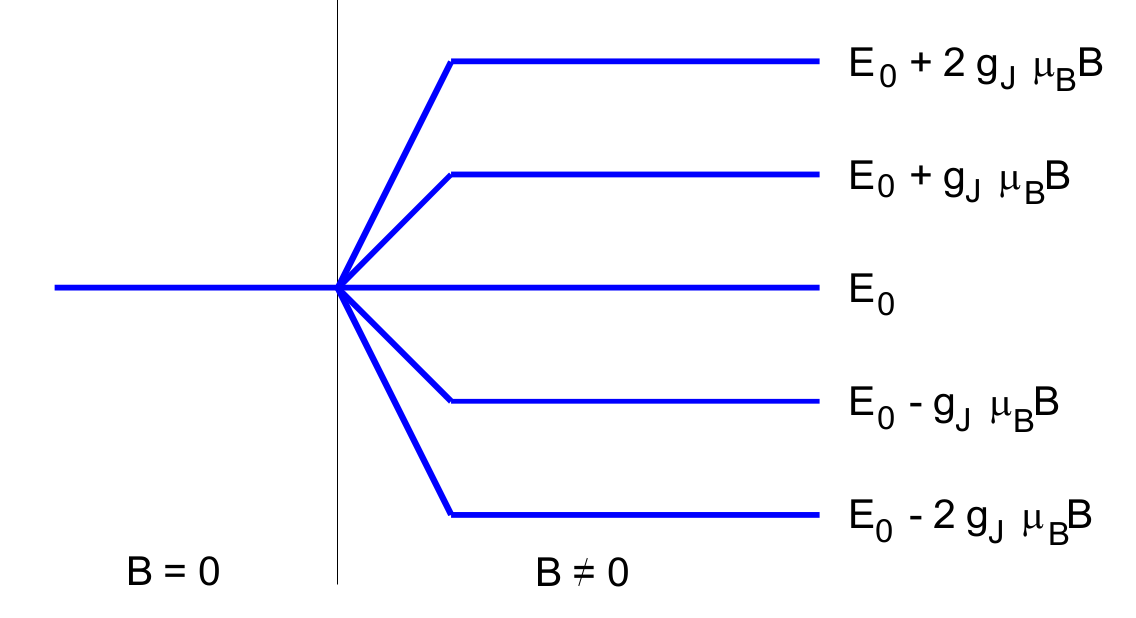
\includegraphics[width=0.6\textwidth]{pics/energieaufspaltung_magnetfeld.png}
  \caption{Energieaufspaltung der Energieniveaus unter Einfluss eines äußeren Magnetfeldes $\vec{B}$ \cite{anleitung27}.}
  \label{fig: energie_magnet}
\end{figure}
\FloatBarrier

Durch die Aufspaltungen entstehen neue mögliche Übergange im Atom, die durch Auswahlregeln festgelegt werden.

\subsection{Auswahlregel und Polarisation}
Die Herleitung der Auswahlregeln soll im Folgenden kurz skizziert werden.
Betrachtet wird zunächst eine Lösung der zeitabhängigen Schrödingergleichung
\begin{equation}
  \label{eq:s_gleichung}
  -\frac{\hbar^2}{2m}\Delta \Psi\left(\vec{r},t\right) + U  \Psi\left(\vec{r},t\right) + \frac{\hbar}{\map{i}} \frac{\partial}{\partial t}  \Psi\left(\vec{r},t\right)=0.
\end{equation}
Welche gegeben ist durch eine Ebene-Welle
\begin{equation*}
  \Psi_{\alpha}\left(\vec{r},t\right)=\Psi_{\alpha}\left(\vec{r}=0,t=0\right)\map{exp}\left(-\frac{\map{i}}{\hbar}E_\alpha t\right).
\end{equation*}
mit den Energiewerten $E_\alpha$. Der Index $\alpha$ bei soll andeuten das die Wellenfunktion
$\Psi_\alpha$ von den Quantenzahlen $n_\alpha$, $l_\alpha$ und $m_\alpha$ abhängt.
Um den Zustandsübergang von zwei einzelnen Energieniveaus $E_\alpha$ bzw. $E_\beta$ zu betrachten,
Superpositionieren wir die jeweiligen Wellengleichungen und erhalten
\begin{equation*}
    \Psi\ua{ges}(\vec{r},t)=C_\alpha\Psi_{\alpha}\left(\vec{r}=0\right)\map{exp}\left(-\frac{\map{i}}{\hbar}E_\alpha t\right)+C_\beta\Psi_{\beta}\left(\vec{r}=0\right)\map{exp}\left(-\frac{\map{i}}{\hbar}E_\beta t\right).
\end{equation*}
Aus den jeweiligen Dipolmomenten der verschiedenen Raumrichtungen $x_i, i=1,2,3$
\begin{equation*}
  D_i=-\map{e_0}\int x_i \Psi^*\ua{ges}\Psi\ua{ges} \dv{V} \qquad i=1,2,3
\end{equation*}
lassen sich dann die Auswahlregeln bestimmen.
Das Resultat der Rechnung ist, das sich die Quantenzahl $m$ zweier Zustände
nur wie folgt unterscheiden dürfen:
\begin{equation}
  \label{eq:auswahlregeln}
  \Delta m=0 , \pm 1
\end{equation}
Weiter kann eine Aussage über die Polarisation des emittierten Lichts getroffen werden.
Ist $\Delta m=0$ so schwingt der Dipol parallel zur Magnetfeldrichtung, dadurch wird \emph{linear polarisiertes} Licht
ausgestrahlt. Bei $\Delta m=\pm 1$ wird ziruklarpolarisiertes Licht emittiert, ebenfalls parallel zum Magnetfeld.

\section{Der normale und annomale Zeeman-Effekt}

\subsection{Der normale Zeeman-Effekt}
Es wird immer dann vom \emph{normalen} Zeeman-Effekt gesprochen, wenn der Elektronspin $S=0$ ist.
Für diesen Spezialfall ist der Lande-Faktor $\map{g_J}=1$ für alle Quantenzahlen $L$ und $J$.
Die Verschiebung der Energieniveaus ist somit gegeben durch
\begin{equation}
  \label{eq: energie_normaler_zeeman}
  \Delta E=m\map{\mu_B}B \qquad m\in\left[-J,J\right].
\end{equation}
Ein Beispiel dazu ist in Abbildung \ref{fig: energie_normaler_zeeman} zu sehen.
\FloatBarrier
\begin{figure}[h]
  \centering
  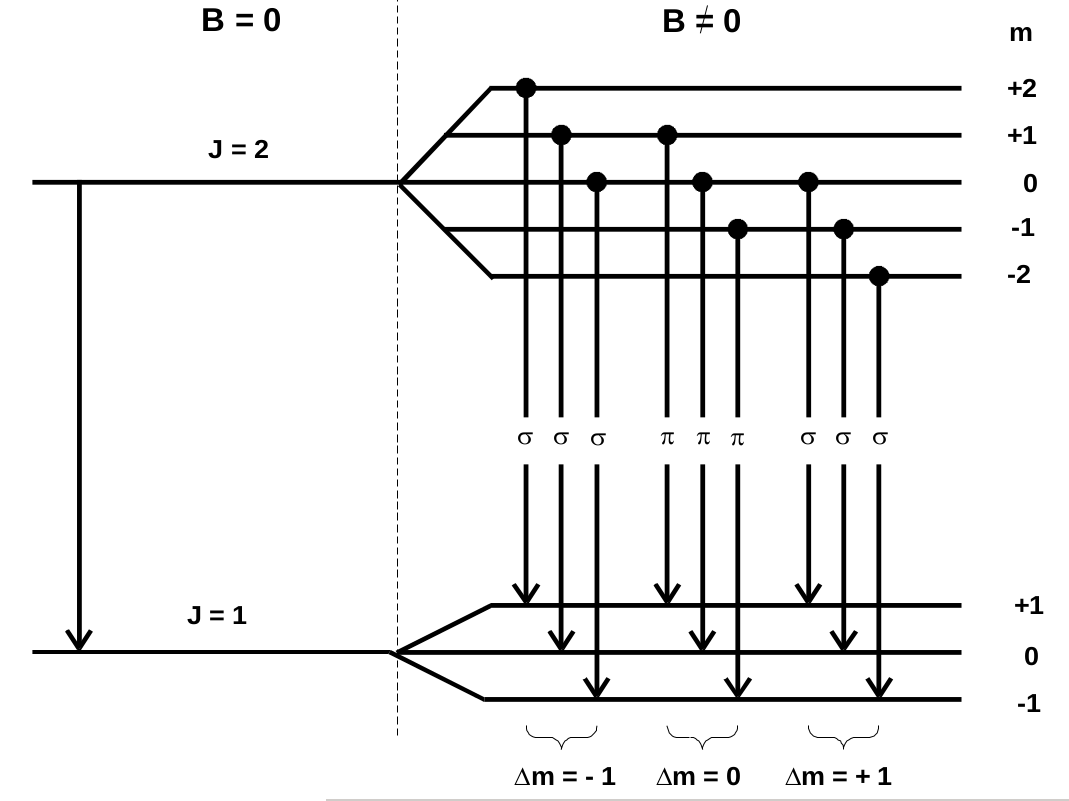
\includegraphics[width=0.6\textwidth]{pics/enerieaufspaltung_normaler_zeeman.png}
  \caption{Beispiel einer Energieaufspaltung beim normalen Zeemaneffekt \cite{anleitung27}.}
  \label{fig: energie_normaler_zeeman}
\end{figure}
\FloatBarrier
Ebenfalls ist in der Abbildung die Polarisationskonvention vermerkt.
Übergänge mit einem $\sigma$ emittieren zirkulär polarisiertes Licht, die mit einem
$\pi$ linear polarisiertes Licht.
Bei der Untersuchung des ausgestrahlten Lichtes muss die Polarisation beachtet werden (vgl. Abbildung \ref{fig: beobachtung_energie}), denn
je nach Polarisation lassen sich nur bestimmte Übergänge beobachten.
\FloatBarrier
\begin{figure}[h]
  \centering
  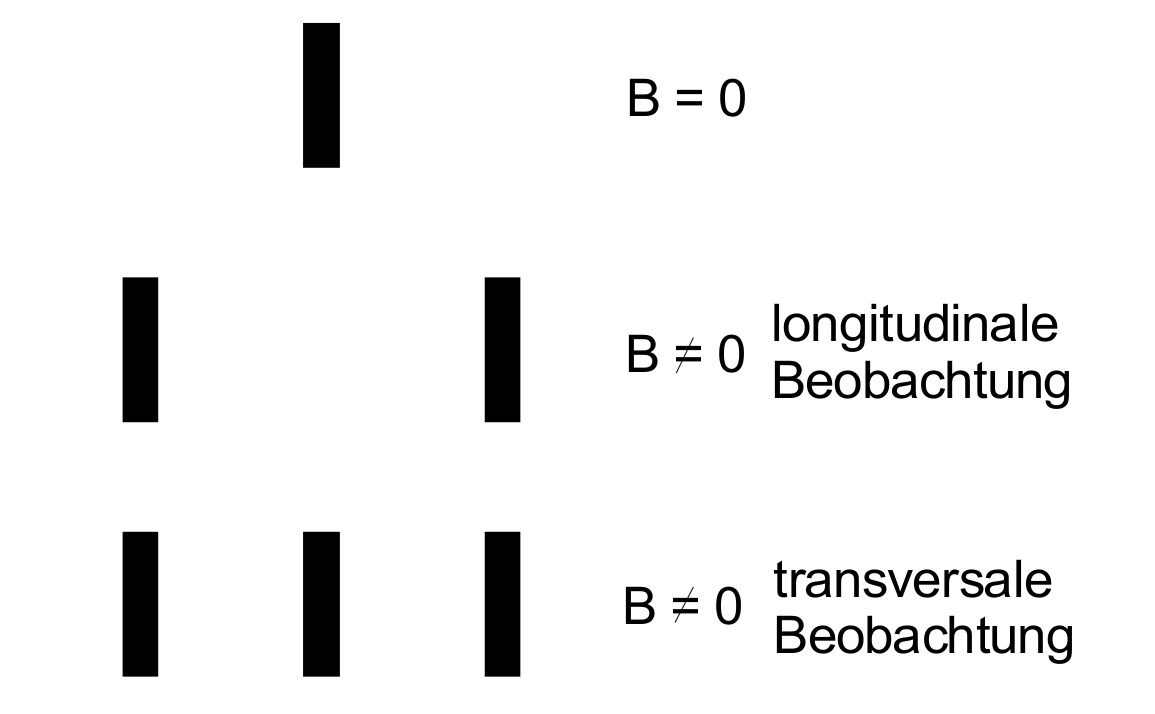
\includegraphics[width=0.6\textwidth]{pics/beobachtung_energie.png}
  \caption{Unterschiedliche Aufspaltungsbilder bei verschiedenen Beobachtungswinkel, auf Grund der Polasirations des emitierten Lichtes \cite{anleitung27}.}
  \label{fig: beobachtung_energie}
\end{figure}
\FloatBarrier

\subsubsection{Der anomale Zeeman-Effekt}
Ist der Elektronspin ungleich null, so spricht man vom \emph{anomalen} Zeeman-Effekt.
Ebenso wie beim normalen Zeeman-Effekt gelten die Auswahlregeln $\Delta m=0, \pm 1$.
Jedoch ist hier die Energiedifferenz, bei einem Übergang von $E_2$ nach $E_1$,
abhängig von den Quantenzahlen $J$, $L$ und $m$
\begin{align}
  E&=\left(m_1\map{g}\left(J_1,L_1,m_1\right)-m_2\map{g}\left(J_2,L_2,m_2\right)\right)\map{\mu_B}B+E_0 \notag \\
  E&=g_{i,j}\map{\mu_B}B \label{eq:energie_anomale_zemman}\\
\shortintertext{mit}
g_{i,j}:\!\!&=m_1\map{g}\left(J_1,L_1,m_1\right)-m_2\map{g}\left(J_2,L_2,m_2\right)\label{eq: faktor_gij}.
\end{align}
Eine beispielhafte Aufspaltung ist in Abbildung \ref{fig: energie_aufspaltung_annomaler} dargestellt.
\FloatBarrier
\begin{figure}[h]
  \centering
  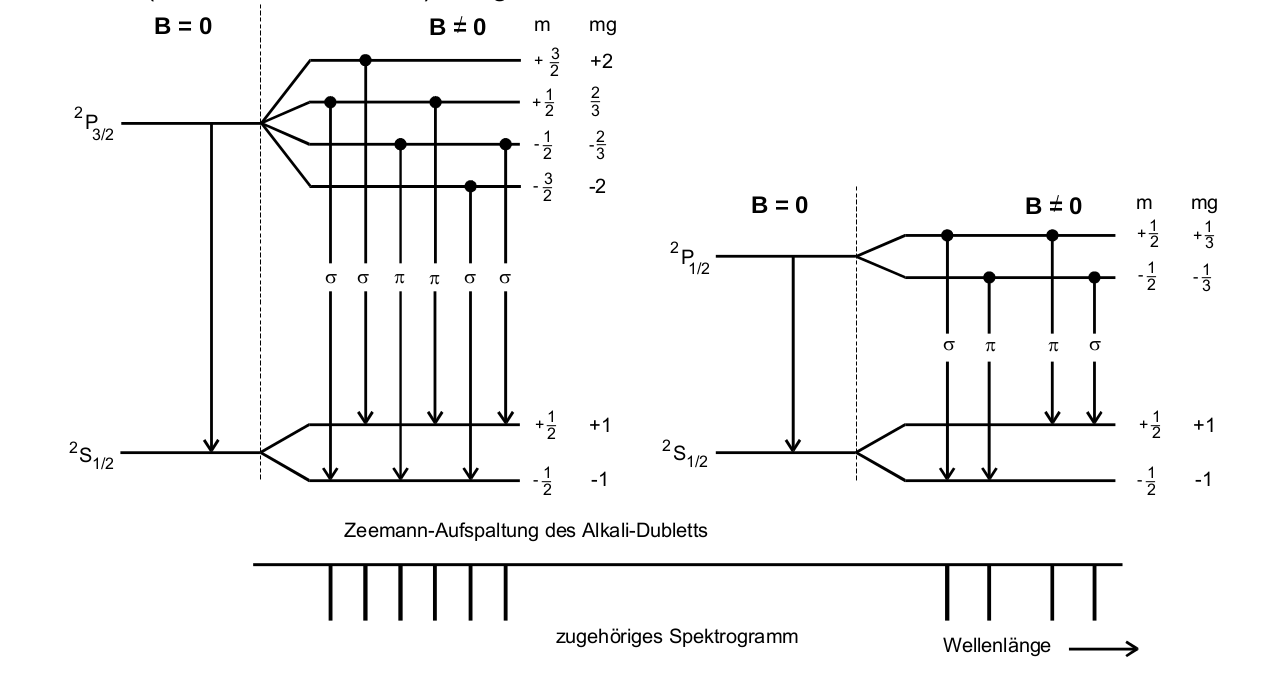
\includegraphics[width=0.8\textwidth]{pics/energieaufspaltung_annomaler.png}
  \caption{Energieaufspaltung beim anomalen Zeeman-Effekt am Beispiel eines Alkali-Duplets \cite{anleitung27}.}
  \label{fig: energie_aufspaltung_annomaler}
\end{figure}
\FloatBarrier
